\appendix
\begin{center}
  \section{人员职责与分工}
\end{center}

\begin{itemize}
  \item 叶晓军:组长,主要负责项目人员组织、进度管理、系统业务逻辑设计
  \item 杨曦华:主要负责系统前端设计
  \item 柯毅豪:主要负责系统后台设计、系统部署
  \item 钟宇腾:主要负责系统架构设计、代码管理
  \item 系统测试与性能调优由全体成员共同完成。
\end{itemize}


\newpage

\begin{center}
  \section{项目开发使用的技术说明}
\end{center}

\subsection{系统架构}
\begin{itemize}
  \item Django Web~框架(项目主页:https://www.djangoproject.com/)
  
  \CJKindent 本系统基于~django web~框架进行开发。~Django Web~框架是一个高级~Python\footnotemark[1] Web~框架,提供~ORM (~Object-relational mapper)~方法,可以完全使用~Python~来定义数据库的表及其元素,并封装了大量的数据库访问~API~,把数据库元素映射为~Python~内部类型,兼容多种数据库后台;提供~Template~系统,可以在~HTML~中嵌入~Python~代码便于服务器动态生成页面;提供缓存模块,提高服务器运行效率。
  
  \item Bootstrap前端框架与交互组件集(项目主页:http://twitter.github.com/bootstrap/)
  
  \CJKindent 本系统前端基于~Bootstrap~模板进行开发。~Bootstrap~是用于快速开发~Web~应用的前端工具包。它是一个~HTML, CSS, JavaScript~的集合,它使用了最新的浏览器技术,给~Web~开发提供了时尚的版式、表单、按钮、表格、网格系统等等。
  
  \item PostgreSQL数据库
  
  \CJKindent 我们的项目使用~PostgreSQL~数据库作为数据库后台,~PostgreSQL~是自由的对象-关系数据库服务器(数据库管理系统),在灵活的~BSD~许可证下发行。~PostgreSQL~使用~SQL~语言来在执行资料的查询。这些资料通过连外键联系在一起,以一系列表格的形式存在。~PostgreSQL~相对于竞争者的主要优势,主要的特征为可编程性:对于使用数据库资料的实际应用,~PostgreSQL~让开发与使用的工作,变得更加容易。与~PostgreSQL~配合的开源软件很多,有很多分布式集群软件,如~pgpool~、~pgcluster~、~slony~、~plploxy~等等,很容易做读写分离、负载均衡、数据水平拆分等方案。
  
  \CJKindent 教务系统经常需要处理高并发情形,~PostgreSQL~是多进程的,在并发不高时处理速度略慢于~MySQL~等多线程数据库,但当并发高的时候,对于现在多核的单台机器上,~PostgreSQL~能利用多核处理器的并发处理优势,整体性能优于其它基于多线程的数据库。
\end{itemize}

本系统是一个基于~Web 2.0~架构的系统,前端使用~AJAX (Asynchronous JavaScript and XML)~来动态显示内容和响应用户输入,服务器采用~Django~网络框架处理数据。在处理请求时不返回整个网页而是只返回用~JSON (JavaScript Object Notation)~表示的数据,前端框架处理数据并呈现,不刷新整个页面而只更新页面的部分内容。

采用此架构可以节约网格资源,在服务器处理大量情求时(如选课时期),可以节约服务器资源和网络带宽,提高网站的响应速度,减轻服务器负担。

本系统在设计时充分考虑到跨平台的需要,兼容绝大多数主流的浏览器(包含桌面系统与手持设备系统的浏览器),在呈现时自动检测显示区域分辨率,若检测到是手持设备的分辨率,则会显示一个专门优化过的页面,提升用户体验。

\footnotetext[1]{Python~是一种面向对象的解析性编程语言、动态语言,支持命令式程序设计、面向对象程序设计、函数式编程、面向切面编程、泛型编程多种编程范式,具备垃圾回收功能,能够自动管理储存器使用。语言设计的哲学是“用一种方法,最好是只有一种方法来做一件事”,语法简洁少有岐义,代码可读性高。}

\subsection{代码托管与版本控制}
\begin{itemize}
  \item Git~版本控制系统
  
  \CJKindent Git~是一个由~Linus Benedict Torvalds~为了更好地管理~Linux~内核开发而创立的分布式版本控制/软件配置管理软件。与常用的版本控制工具~CVS、Subversion~等不同,它使用了分布式版本库,不需要服务器端软件支持,使源代码的发布和交流极其方便。~Git~的速度很快,这对于诸如~Linux kernel~这样的大项目来说自然很重要。~Git~最为出色的是它的合并跟踪(~merge tracing~)能力。
  
  \item GitHub
  
  \CJKindent GitHub~是一个基于互联网、使用~Git~版本控制系统的项目存取服务,提供了诸如~feeds~,~followers~,开发者的工作网络图表等统计服务。根据在2009年的~Git~用户调查,~GitHub~是最流行的~Git~存取站点。
  
  \CJKindent 我们的项目托管于~GitHub~,地址为~https://github.com/zonyitoo/SYSUEduAdminSystem~,使用~Git~版本控制系统来进行版本控制和软件配置管理。
\end{itemize}

\newpage
\begin{center}
  \section{开发总结与心得感悟}
\end{center}

\subsection{版本控制系统图表分析}
\begin{figure}[H]
   \centering 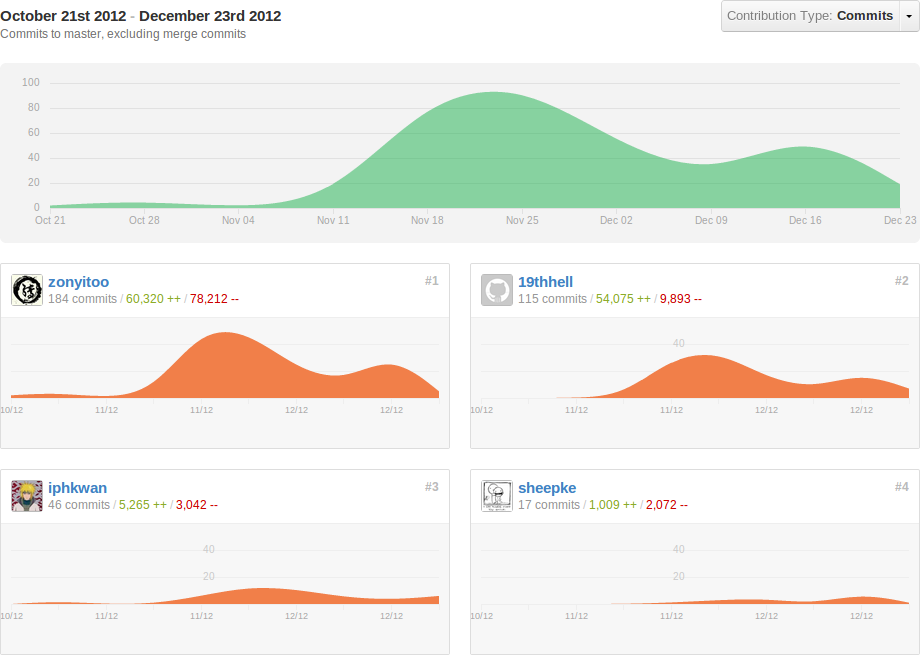
\includegraphics[width=\textwidth]{img/contrib.png}
   \caption{项目成员贡献及项目提交数与时间关系图}
\end{figure}

上图中,帐号与成员的对应关系为:钟宇腾(~zonyitoo~)、杨曦华(~19thhell~)、叶晓军(~iphkwan~)、柯毅豪(~sheepke~)。我们的项目从2012年10月21日开始编写,至2012年12月23日完成。在2012年11月20日前后进行基础框架搭建,并推出~Alpha~测试版,在2012年12月16日前后对于系统细节修补及加入新功能,推出~Beta~测试版。

钟宇腾(~zonyitoo~)是项目代码的管理员,主要负责项目文件树管理及架构设计,因此提交数(~Commits~)最多,增加了60320行代码,删除78212行代码;杨曦华(~19thhell~)是网页前端开发者,主要负责网页前端设计,有115次提交,增加了54075行代码,删除9893行代码;叶晓军(~iphkwan~)是组长,主要负责项目进度管理,有46次提交,增加5256行代码,删除3042行代码;柯毅豪(~sheepke~)是系统后台开发者,主要负责后台服务器响应代码编写及服务器维护及测试,有17次提交,增加1009行代码,删除2072行代码。全组所有成员在基本分工下互相合作,并没有很绝对的分工界线。

\begin{figure}[H]
   \centering 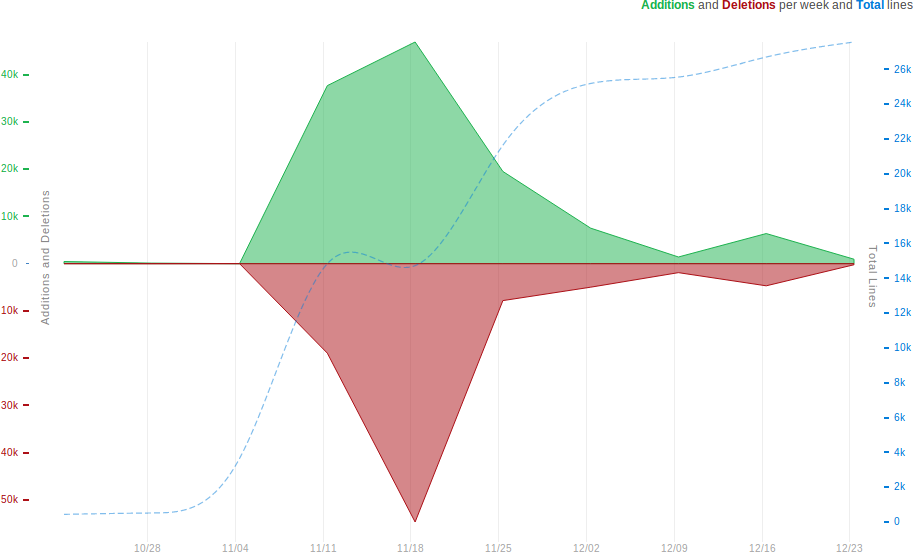
\includegraphics[width=\textwidth]{img/code_freq.png}
   \caption{项目代码变化图}
\end{figure}

图中虚线是代表代码行数的变化与时间的关系,2012年12月23日后代码行数超过了2.6万。中央横线以上的图中,高度代表该时间段增加的代码行数;中央横线以下的图中,高度代表该时间段被删除的代码行数,总体体现了代码增加的速度。\vspace{2em}

项目托管主页:https://github.com/zonyitoo/SYSUEduAdminSystem

项目统计图:https://github.com/zonyitoo/SYSUEduAdminSystem/graphs

\subsection{个人总结与感悟}
\begin{itemize}
  \item 叶晓军
  
  \CJKindent 本学期初,本人联系上杨曦华、柯毅豪和钟宇腾三位编程牛人组队,并十分荣幸地被推举为组长,开始了软件工程课程项目的设计与开发。作为项目的负责人,在项目中我更多地负责人员的组织与开发进度的管理。
  
  \CJKindent 在项目开发过程中,我遇到的第一个挑战就是,我和小组各成员都不甚了解网站开发技术。因此,在项目起步阶段,如何确定网站的开发框架、合理地分工学习网站开发技术变得十分重要。在与小组成员的多次讨论交流中,我大致了解到,杨曦华擅长图像的设计与处理;柯毅豪对系统后台有一定的认识,擅长系统的部署;钟宇腾热衷于追求最新的技术,拥有敏锐的技术触觉;而至于我自己,大学前两年的ACM/ICPC锻炼经历让我具备了不错的逻辑分析设计能力与代码查错能力。由于小组中我和钟宇腾之前已熟悉Python语言,为了降低学习成本,我们敲定了网站后台使用由Python语言开发的、当前业界新兴起来的Django框架,由柯毅豪和钟宇腾负责。同时,擅长页面设计的样曦华毫无疑问地负责网站前端的设计,开始了html/css/ajax等相关网页设计技术的深入学习。为了沟通好前后端,虽不深入,但作为组长的我必须对所有技术都有所涉猎,在开发中后期主力负责代码的查错调优。
  
  \CJKindent 作为一个项目团队,成员间的沟通协作非常重要。如果我们四人分别在各自的地方进行编码,利用qq、gmail等网络通讯工具进行交流协作,效率将十分低下。因此,我选择了四人都空余的每周周五下午,到学院楼的学术讨论室,集中进行项目核心功能代码的编写。集中编码的另一个好处就是,通过聆听小组成员的技术讲解,我们可以更加高效地学习自己之前不熟悉的技术。此外,技术讲解也是一个锻炼自己表达能力的过程,在讲解讨论中,讲解人也能加深对技术的认识,整个项目的编码质量也会得到提高。
  
  \CJKindent 回顾整个软件工程过程,从立项、文档编写,到代码开发、调试部署,我受益匪浅。在文档编写阶段,我体会到文档格式严谨的重要性,通过对图表、文字表述的反复修改,我提高了文字表述能力;在代码开发阶段,我学习了许多前沿的网站开发技术,这对我日后个人职业发展具有深远影响;在代码查错调优阶段,我体会到工程代码与ACM编程比赛的编码的不同,工程编码需要程序员更加注重代码的可读性与可维护性……最后,衷心感谢衣杨老师对我、对我们小组项目的指导和帮助,您给我们指出的不足让我们看到了自己发展的潜力;感谢三位给力的队友对本人工作的支持和配合,能在融洽的团队开发氛围下互相学习、一起工作是一种美妙的享受。
  
  \item 杨曦华
  
  \CJKindent 通过本次项目实践,我主要的收获是学习并初步掌握了如何对一个问题进行需求分析、如何用模块化的方式去进行系统的架构设计、如何以团队方式进行项目开发。在这次项目的开发过程中,我主要负责的是前端的工作。
  
  \CJKindent 通过这次项目开发经历,我了解到一个项目开发的速度和质量与这个项目的文档完善程度是有很大关系的,以系统结构设计文档为例,这次项目的结构设计文档的前几个版本有一些地方考虑得并不周到,以至于在我们实际进行开发时遇到一些需要在架构上进行大量改动才能保持系统健壮性的设计。这种改动出现在项目开发的前期或许不会让成本出现过大的提升,但如果在项目开发的后期才发现因为结构设计不够妥当而需要对结构进行大改甚至是完全重构,这对项目开发的进度无疑会有灾难性的影响。工欲善其事必先利其器,要做好一个项目就必须对每一步都认真对待和充分考虑。
  
  \CJKindent 对项目完成质量影响很大的另一个因素是对各种新技术的使用,例如我们开发的系统采用Django作为服务器框架,使用Python语言进行后台开发,与前端的通信主要通过Json数据包而不是直接发送网页,这种搭建方式不但可以提高系统的运行效率,也可以更好地区分前端和后台的工作,更重要的是使得代码具有很好的可读性和可维护性,这些特性有许多是PHP等出现较早的语言难以完美地体现的。同时,采用Github进行代码的版本控制和托管,这种方式很好地加强了团队成员之间的交流,而不是每个人完全独立地修改自己的代码,有不少漏洞和错误正是通过这种团队交流才得以发现和修复的。
  
  \CJKindent 通过本次项目实践,我不但学习到了许多新技术,也体会到团队合作的许多优势,这些经历对我来说是很有用的积累,而我能在一次项目开发中得到这么多的收获,与衣杨老师的教导和与其他几位团队成员的交流是分不开的。
  
  \item 柯毅豪
  
  \CJKindent 在学习软件工程之前,我编写的程序大多数都是算法和数据交织在一起,尽管后来将数据独立出来保存在文件中,不过为了处理输入输出的格式问题,依旧需要浪费很多时间。在学习了MVC架构之后,更加能够理解数据库系统在大型软件项目中的重要性。
  
  \CJKindent 在这个学期编写教务系统这个项目的过程中,我学到了很多不同方面的东西。以前写程序时,不会先编写文档,而是直接开始构思代码,虽然看起来节省了时间,不过到了中间就会发现原来的构思有缺陷,需要推倒重来。而通过小组成员间讨论软件架构的组成,然后再一步一步抽象出各个类,这种方法使得后面的实现过程更加顺畅,也降低了重构发生的可能性。
  
  \CJKindent 在实现教务系统的过程中,小组决定使用Python语言和Django框架。我之前并没有接触过Python语言和Django框架。不过在浏览了相关的Python书籍和Django手册后,再结合小组成员已有的代码,我也能够做到边学边用,逐渐完成了选课退课和课程筛选部分的后台代码编写工作。这三个月的过程让我感受到,已有多少知识和技能并不是最重要的,关键是有足够的学习能力,在给定的时间内学会并应用新的知识。
  
  \CJKindent 软件工程项目和之前个人的小项目相比,更注重团队合作。这次项目是我第一次依赖Git和Github进行代码的版本管理。团队中的每一个人提交了代码之后,如果备注了哪个地方存在bug,大家很快就会互相讨论如何解决,而不是仅靠一个人的力量苦苦挣扎。这种团队合作的氛围使得工作的效率大大提升。
  
  \item 钟宇腾
  
  \CJKindent 在本次软件工程的项目小组中,我主要负责架构设计、项目管理、服务器后台软件编写。
  
  \CJKindent 我们小组的成员都喜欢尝试新技术,比如在编写分析与设计文档时,我们为了让大家都更方便地参与到文档的编写中去,采用了在线文档协作平台—— Google Docs进行文档的编写,可以多人同时在线对一个文档的各个不同部分进行编写,提高了工作效率,在自己编写文档的同时也能让其它组员检查错误,提高文档的质量;在代码编写时,我们使用了版本控制工具,使得每个成员都能及时得到最新的代码,及时发现和修正错误,出现重大错误时可以方便回滚到历史上某个正常版本,有利于迭代开发,提高编码效率和软件质量;我们的所有代码都托管到网站上,所有成员都可以对某一次的提交留言,方便成员间交流合作;还有全新的数据库后台系统、全新的编程语言……得益于使用当前比较流行的新技术,使我们能够在两个半月的时间里顺利完成项目的开发与测试工作,采用开源技术使我们从开源社区中获益良多。
  
  \CJKindent 在本次软件项目开发过程中,我收获最大的是体验团队合作的氛围。在合作过程中,成员间出现的各种分歧是影响开发进度和团队凝聚力的重要因素,沟通是解决分歧的重要手段。通过互相沟通,理解对方的立场,团队成员相互磨合,最后得出大家都满意的结果。在讨论中的思维碰撞也有利于得出更优的解决方案,有利于提高软件质量。
  
  \CJKindent 通过本次软件工程的项目,我在学习到许多的新技术之余,更大的收获是团队的合作经验。新技术有利于我了解当今时代信息技术的发展方向以及掌握更多更有用的技术,团队合作的经验则有利于我未来真正加入到团队中时更好的融入团队、发挥自己的能力。因此本次项目实践于我来说是一次非常宝贵的经验,感谢衣杨老师及我的队友。

\end{itemize}
